
%%%%%%%%%%%%%%%%%%%%%%%%%%%%%%%%%%%%%%%%%%%%%%%%%%%%%%%%%%%%%%%%%%%%%%%%%%%%%%%%
%%%%%%%%%%%%%%%%%%%%%%%%%%%%%%%%%%%%%%%%%%%%%%%%%%%%%%%%%%%%%%%%%%%%%%%%%%%%%%%%
\section{Definições relativas as danças a dois}

Antes de iniciar as explicações no capítulo, 
é necessário partir desde uma linguagem comum;
com este propósito, 
significados de algumas palavras bem definidas na literatura são mostrados a continuação:
 
\begin{definition}[Princípio:] 
\index{Princípios}
\label{def:Principio}O Dicionário Priberam da Língua Portuguesa \cite{priberamprincipio} define princípio como:
Frase ou raciocínio que é base de uma arte, de uma ciência ou de uma teoria.
Adicionalmente o Dicionário Online de Português, DICIO \cite{dicioprincipio}, define princípio como:
Informação básica e necessária que fundamenta uma seção de conhecimentos.
Exemplo:princípios da matemática.
\end{definition}

\begin{definition}[Casal:] 
\index{Casal}
\label{def:Casal} O Dicionário Priberam da Língua Portuguesa \cite{priberamcasal} define casal como:
Par formado por um macho e uma fêmea.
Exemplo: casal de cavalos, casal de pombas, casal de humanos.
\end{definition}

\begin{definition}[Par:] 
\index{Par}
\label{def:Par} O Dicionário Priberam da Língua Portuguesa \cite{priberampar} define par como:
Igual, semelhante, parceiro.
Cada uma das pessoas que constituem uma dupla na dança.
\end{definition}


%%%%%%%%%%%%%%%%%%%%%%%%%%%%%%%%%%%%%%%%%%%%%%%%%%%%%%%%%%%%%%%%%%%%%%%%%%%%%%%%
\subsection{Definições sobre condução nas danças a dois}
Usando como base os significados mostrados anteriormente, 
serão descritos alguns termos muito utilizados na dança\footnote{
Para as definições, foi priorizado o uso da palavra par sobre a palavra casal,
para poder definir às entidades dançantes independentemente do sexo dos participantes.}.
Assim,  são propostas as seguintes definições:

\begin{definition}[Paradigma da condução (Dança):] 
\index{Condução} 
\label{def:ParadigmaConducao} 
Este é um modelo de dança a dois usado na \hyperref[def:DancaSalao]{\textbf{dança de salão}},
\hyperref[def:DancaSocial]{\textbf{dança social}}, etc. 
E indica que entre as pessoas que conformam a dança, 
existe uma transmissão de informação relativa à movimentação e as pausas, no \hyperref[def:Par]{\textbf{par}} dançante; 
de modo que, a informação tem um fluxo unidirecional no médio de transmissão,
que vá desde o \hyperref[def:Condutor]{\textbf{condutor}} (Transmissor/Tx) 
ate o \hyperref[def:Seguidor]{\textbf{seguidor}} (Receptor/Rx),
ver Figura \ref{fig:paradigmaconducion}. 
\end{definition}
\index{Condutor} 

\begin{figure}[!ht]
     \centering
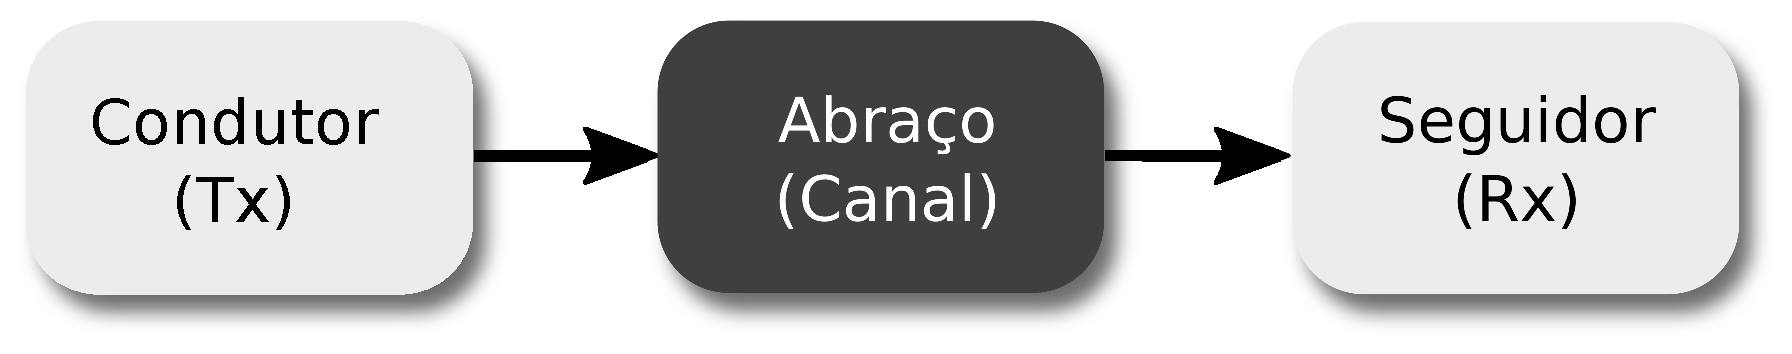
\includegraphics[width=0.75\textwidth]{chapters/cap-normas/modeloconducao.eps}
\caption{Fluxo da informação na condução}
\label{fig:paradigmaconducion}
\end{figure}

Seguindo a desigualdade de processamento de dados (do inglês ``data-processing inequality''),
qualquer processamento efetuado sobre a informação nunca nos proporcionará mais informação da recebida;
é dizer, qualquer processamento da informação só produzirá perdas,
ou num caso ideal obteremos a mesma informação  \cite[pp. 34]{cover2006elements}.
Assim, quando utilizamos o \hyperref[def:ParadigmaConducao]{\textbf{paradigma da condução}} na nossa dança,
as transformações efetuadas pelo meio de transmissão (o abraço), 
só podem produzir perdas sobre a informação transmitida;
pelo que devemos ter muito cuidado, no nosso abraço de dança,
procurando a \hyperref[def:brazosfirmes]{\textbf{firmeza de braços}}, 
para que a informação enviada pelo \hyperref[def:Condutor]{\textbf{condutor}} 
chegue ao \hyperref[def:Seguidor]{\textbf{seguidor}} o mais integra possível.

Assim, o 100\% de eficiência na transmissão ``bruta'' da informação
é  um alvo teórico possível; porem, pouco provável de acontecer na prática.
Entretanto, é possível atingir valores próximos ao 100\% de eficiência,
se agregamos um boa quantidade de redundância na informação transmitida na condução  \cite[pp. 184,219]{cover2006elements}.
 

\begin{definition}[Condutor (Dança):] 
\index{Condutor} 
\label{def:Condutor} 
A pessoa que tem o papel de conduzir ou propor o movimento ao \hyperref[def:Seguidor]{\textbf{seguidor}}. 
O objetivo técnico das pessoas que optam por este rol na dança, é chegar 
a ter a sensibilidade necessária para entender onde está localizado espacialmente, 
e como distribui o peso do corpo, o \hyperref[def:Seguidor]{\textbf{seguidor}}; 
de modo que seja possível para o condutor aplicar sobre o \hyperref[def:Seguidor]{\textbf{seguidor}}, 
uma mistura de indicações, forças e torções,  
para provocar os movimentos ou pausas desejadas;
chama-se a isto saber conduzir.
Sinônimos de condutor: Líder (Dança).
\end{definition}

\begin{definition}[Seguidor (Dança):] 
\index{Seguidor} 
\index{Conduzido} 
\label{def:Seguidor} 
A pessoa que recebe a condução e proporciona uma resposta corporal. 
O objetivo técnico das pessoas que optam por este rol na dança, é chegar 
a ter a sensibilidade necessária para entender e incorporar as conduções,
independentemente de quem seja a pessoa que aplique a condução;
chama-se a isto ser conduzível.
Sinônimos de seguidor: \textbf{Conduzido}.
\end{definition}

O \hyperref[def:ParadigmaConducao]{\textbf{paradigma da condução}},
 descreve um modelo de transmissão unidirecional de informação com emissor fixo;
entretanto, como é visto na Figura \ref{fig:tiposcomunica}, 
existem outros métodos de transmissão de informação que podem ser explorados 
sobre um único canal de comunicação.
\begin{figure}[!ht]
     \centering
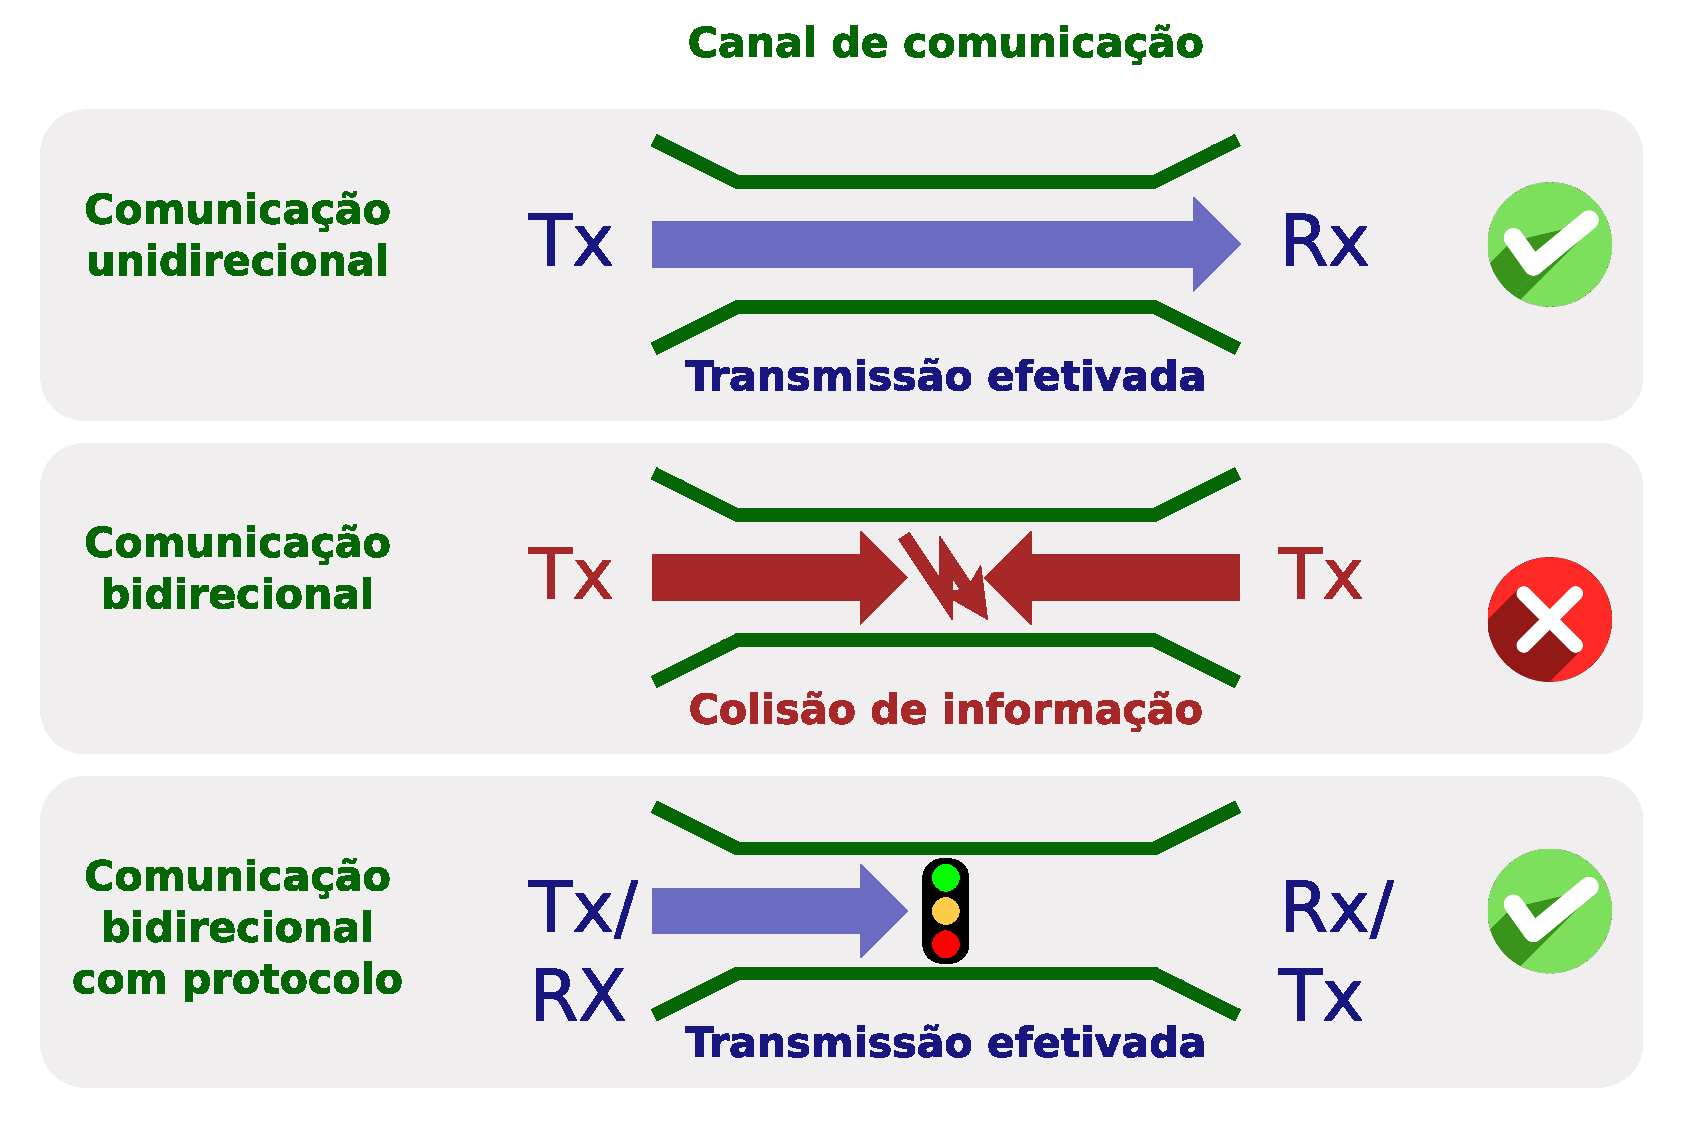
\includegraphics[width=0.95\textwidth]{chapters/cap-normas/tiposcomunica.eps}
\caption{Comunicação unidirecional vs. bidirecional}
\label{fig:tiposcomunica}
\end{figure}
%%%%%%%%%%%%%%%%%%%%%%%%%%%%%%%%%%%%%%%%%%%%%%%%%%%%%%%%%%%%%%%%%%%%%%%%%%%%%%%%
\subsection{Definições sobre tipos de danças a dois}

Nas definições desta seção, foram tomados dois conceitos do artigo 
``Conceitos e definição de Dança de Salão'' \cite{Zamoner2012};
modificações foram feitas para adaptar estas definições aos conceitos de 
\hyperref[def:Condutor]{\textbf{condutor}} e \hyperref[def:Seguidor]{\textbf{seguidor}}, 
usados ao longo deste livro.

\begin{definition}[Dança social:]
\index{Dança social} 
\label{def:DancaSocial} 
É uma dança com fim recreativo de prática social, não cênica, nem competitiva, 
que não tem um interesse artístico, histórico, geográfico ou técnico; 
que se universaliza e consiste na movimentação dos corpos do \hyperref[def:Par]{\textbf{par}} de dança  \cite{Zamoner2012}, 
onde existe o rol do \hyperref[def:Condutor]{\textbf{condutor}} 
e do \hyperref[def:Seguidor]{\textbf{seguidor}} (papeis intercambiáveis), 
ate onde o nível técnico do par o permita.
\end{definition}

\begin{definition}[Dança de salão:]
\index{Dança de salão}
\label{def:DancaSalao}  
É uma arte que procura conservar suas características técnicas, 
sua origem histórica e geográfica, e se universaliza em práticas sociais. 
Esta arte consiste na interpretação improvisada da música por médio dos movimentos 
dos corpos de um \hyperref[def:Par]{\textbf{par}} de dança \cite{Zamoner2012}, 
utilizando o \hyperref[def:ParadigmaConducao]{\textbf{paradigma da condução}} .
\end{definition}

%%%%%%%%%%%%%%%%%%%%%%%%%%%%%%%%%%%%%%%%%%%%%%%%%%%%%%%%%%%%%%%%%%%%%%%%%%%%%%%%
\subsection{Definições sobre o abraço nas danças a dois}

\begin{definition}[Firmeza de braços (Dança):]
\index{Firmeza de braços}
\label{def:brazosfirmes} 
Que o \hyperref[def:Condutor]{\textbf{condutor}} e \hyperref[def:Seguidor]{\textbf{seguidor}}
tenham os braços firmes, não implica fazer força pra submeter ao par;
e sim, ativar os músculos o mínimo e necessário para manter a posição relativa e postura dos braços.
de modo que a informação de condução passe através dos braços no abraço, 
e chegue com fidelidade ao corpo do seguidor.

Outra forma de descrever a firmeza dos braços, 
é indicando que esta ação implica ter uma ativação muscular e auto controle, 
para suprimir conscientemente alguns graus de liberdade que existem nas articulações nos braços, 
dependendo da situação e do estilo de dança.
\end{definition}




Na Figura \ref{fig:modelobrazo} podemos ver um modelo simplificado de um braço,
usando 5 graus de liberdade:
\begin{itemize}
\item 2 graus de liberdade, $\theta_1$ e $\theta_2$, nos movimentos de rotação e abertura do ombro.
\item 1 grau de liberdade, $\theta_3$, no movimento de flexão no cotovelo.
\item 1 grau de liberdade, $\theta_4$, no movimento de rotação no antebraço.
\item 1 grau de liberdade, $\theta_5$, no movimento de flexão no pulso.
\end{itemize}

 

\begin{figure}[!ht]
     \centering
     \begin{subfigure}[b]{0.31\textwidth}
         \centering
         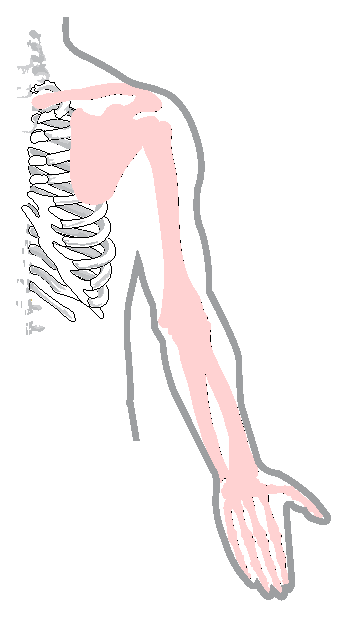
\includegraphics[width=\textwidth]{chapters/cap-normas/brazo1.eps}
         \caption{Modelo humano}
         \label{fig:modelobrazo1}
     \end{subfigure}
     \hfill
     \begin{subfigure}[b]{0.31\textwidth}
         \centering
         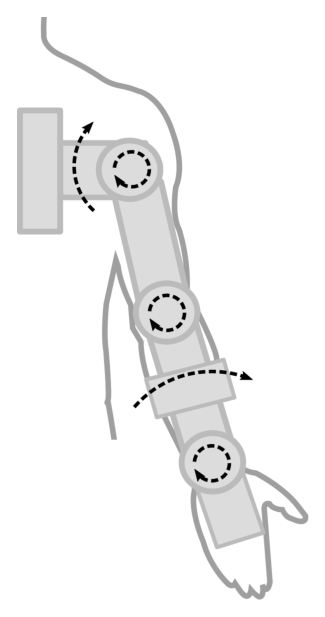
\includegraphics[width=\textwidth]{chapters/cap-normas/brazo2.eps}
         \caption{Modelo mecánico}
         \label{fig:modelobrazo2}
     \end{subfigure}
     \hfill
     \begin{subfigure}[b]{0.31\textwidth}
         \centering
         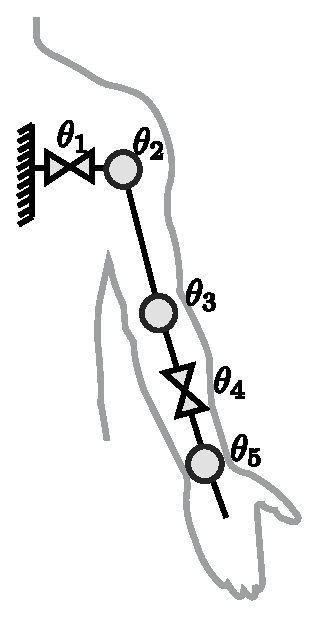
\includegraphics[width=\textwidth]{chapters/cap-normas/brazo3.eps}
         \caption{Modelo teórico}
         \label{fig:modelobrazo3}
     \end{subfigure}
\caption{Modelo de um braço}
\label{fig:modelobrazo}
\end{figure}

Quando iniciamos nosso aprendizado na dança, 
o primeiro grau de liberdade que aprendemos a bloquear de forma inteligente é $\theta_5$ (pulso),
pois é o que instintivamente fazemos quando nos indicam ter os braços firmes.
O grau de liberdade representado por $\theta_4$ (antebraço), geralmente estará livre na nossa dança,
e ajudará a ter uma postura confortável no abraço.
Quando realmente iniciamos a entender, que é ter firmeza do braços,
é quando iniciamos a controlar o grau de liberdade representado por $\theta_3$ (cotovelo);
pois esta articulação permite que nosso par de dança sempre esteja dentro de nosso abraço.
O último nível de nosso aprendizagem para garantir a firmeza de braços,
é controlar consciente e inteligentemente quando bloquear  $\theta_1$ e $\theta_2$ (hombro),
esta articulação é muito descuidada pelos condutores e seguidores,
pois a maioria das pessoas vem como alvo final do seu treinamento,
controlar a articulação do cotovelo. 

\begin{definition}[Abraço de dança:]
\index{Abraço de dança}
\label{def:abracodedanca}  
É um abraço onde o \hyperref[def:Condutor]{\textbf{condutor}} 
rodeia com a mão direita as costas do \hyperref[def:Seguidor]{\textbf{seguidor}},
numa linha meia entre a linha dos ombros e a linha da parte baixa do tórax;
enquanto a mão esquerda, do condutor, segura com o braço semi flexionado a mão direita do seguidor,
colocando ambas mãos a altura do ombro da pessoa mais baixa do \hyperref[def:Par]{\textbf{par}}.
Por outro lado, o seguidor também rodeia com seus braços ao condutor,
de modo que seu braço esquerdo rodeie o braço direto do condutor ate chegar,
na medida do possível, na altura dos ombros. 

É preferível que a palma da mão esquerda do seguidor não esteja apontando ao chão,
para evitar que inconscientemente o seguidor recarregue seu peso no ombro do condutor,
pelo que uma boa alternativa seria que a palma da mão do seguidor aponte a algum ponto no peito do próprio seguidor.

Por motivos similares, é preferível que o cotovelo do braço direito do seguidor,
que segura a mão do condutor,
não aponte ao chão e sim e sim que esteja ligeiramente levantado,
para que não seja esquecido que o peso desse braço ou do corpo não deve ser recarregado no condutor. 
\end{definition}

%%%%%%%%%%%%%%%%%%%%%%%%%%%%%%%%%%%%%%%%%%%%%%%%%%%%%%%%%%%%%%%%%%%%%%%%%%%%%%%%
\subsection{Definições sobre posições corporais  nas danças a dois}

%%%%%%%%%%%%%%%%%%%%%%%%%%%%%%%%%%%%%%%%%%%%%%%%%%%%%%%%%%%%%%%%%%%%%%%%%%%%%%%%
\subsubsection{Classificação seguindo a proximidade dos corpos}

Como mostra a Figura \ref{fig:proximidadeabraco1},
podemos ter pelo menos 3 tipos de posições
para o abraço na dança a dois, 
classificando-os seguindo a proximidade dos corpos.

\begin{figure}[!ht]
     \centering
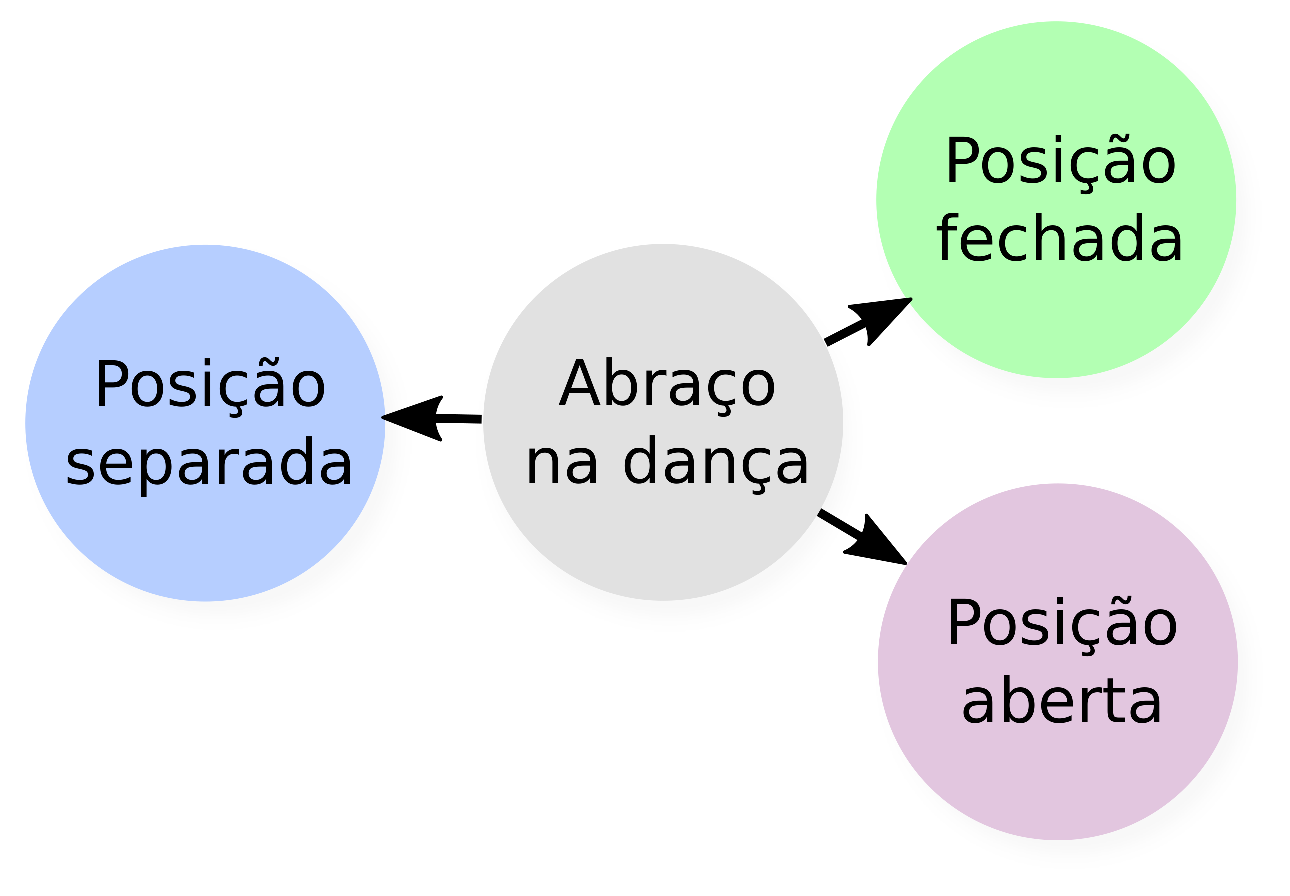
\includegraphics[width=0.7\textwidth]{chapters/cap-normas/proximidadeabraco1.eps}
\caption{Classificação do abraço na dança a dois seguindo a proximidade dos corpos}
\label{fig:proximidadeabraco1}
\end{figure}

\begin{definition}[Posição fechada:]
\index{Abraço de dança!Posição fechada}
\label{def:closed-position}  (do inglês ``closed position'')
As pessoas do \hyperref[def:Par]{\textbf{par}} de dança estão frente a frente, tendo contato no tórax,
realizando um \hyperref[def:abracodedanca]{\textbf{abraço de dança}}; 
cada pessoa olha por cima do ombro direito do outro,
e os dedos dos pés de cada pessoa apontam a outra \cite{fletsher2015improve}.
\end{definition}


\begin{definition}[Posição aberta:]
\index{Abraço de dança!Posição aberta}
\label{def:open-position} (do inglês ``open position'') 
É similar à posição fechada, 
com a diferencia que não se tem contanto entre os tórax do \hyperref[def:Par]{\textbf{par}},
estando estes separados, aproximadamente, 1 palmo de distancia \cite{fletsher2015improve}.
\end{definition}



\begin{definition}[Posição separada:]
\index{Abraço de dança!Posição separada}
\label{def:apart-position} (do inglês ``apart position'') 
As pessoas do \hyperref[def:Par]{\textbf{par}} de dança estão frente a frente;
porem, elas estão tão separadas, 
que não é possível realizar um abraço de dança, 
pelo que o par só se segura por uma ou as duas mãos \cite{fletsher2015improve}.
\end{definition}

%%%%%%%%%%%%%%%%%%%%%%%%%%%%%%%%%%%%%%%%%%%%%%%%%%%%%%%%%%%%%%%%%%%%%%%%%%%%%%%%
\subsubsection{Classificação seguindo as posturas dos corpos}
Se classificamos as posições do par de dança seguindo as posturas dos corpos,
no samba de gafieira, comumente, podemos encontrar os seguintes tipos de posições:

\begin{definition}[Posição de X:]
\index{Abraço de dança!Posição de X}
\label{def:X-position} 
Refere-se a uma posição quando ambas pessoas do \hyperref[def:Par]{\textbf{par}}, 
de dança estão em com o quadril apontando criando linhas paralelas,
o \hyperref[def:Condutor]{\textbf{condutor}}, na linha do lado esquerdo e
o \hyperref[def:Seguidor]{\textbf{seguidor}}, na linha do lado direito.
O par estará formando um \hyperref[def:abracodedanca]{\textbf{abraço de dança}}
que pode ser \hyperref[def:closed-position]{\textbf{fechado}} 
ou \hyperref[def:open-position]{\textbf{aberto}},
de modo que existe dissociação entre o quadril e o tórax,
sendo que os tórax das pessoas do par apontam um ao outro.
\end{definition}

\begin{definition}[Posição frente a frente:]
\index{Abraço de dança!Posição frente a frente}
\label{def:frente-frente-position} 
Refere-se a uma posição quando ambas pessoas do \hyperref[def:Par]{\textbf{par}}, 
de dança estão um frente ou outro,
com a linha do quadril e ombros paralelos entre o 
\hyperref[def:Condutor]{\textbf{condutor}} e
\hyperref[def:Seguidor]{\textbf{seguidor}}.
O abraço de dança pode ter uma posição \hyperref[def:closed-position]{\textbf{fechada}} 
ou \hyperref[def:open-position]{\textbf{aberta}}.
\end{definition}

\begin{definition}[Posição lateral:]
\index{Abraço de dança!Posição lateral}
\label{def:lateral-position}  (do inglês ``side position'') 
O lado direito do \hyperref[def:Condutor]{\textbf{condutor}} e o 
lado esquerdo do \hyperref[def:Seguidor]{\textbf{seguidor}} estão juntos,
enquanto que o lado esquerdo do condutor e o direito do seguidor estão afastados,
de modo que os tórax, das pessoas do \hyperref[def:Par]{\textbf{par}}, formam um angulo de aproximadamente $180^o$;
eles podem ou não as mãos seguradas \cite{fletsher2015improve}
\end{definition}


\begin{definition}[Posição promenade:]
\index{Abraço de dança!Posição promenade}
\label{def:promenade-position}  (do inglês ``promenade position'') 
O lado direito do \hyperref[def:Condutor]{\textbf{condutor}} e o 
lado esquerdo do \hyperref[def:Seguidor]{\textbf{seguidor}} estão juntos,
enquanto que o lado esquerdo do condutor e o direito do seguidor estão afastados,
de modo que os tórax, das pessoas do \hyperref[def:Par]{\textbf{par}}, formam um angulo menor a $180^o$;
é dizer, formam uma posição de V;
eles podem ou não ter as mãos seguradas \cite[pp. 13, 16]{BallroomDancing1992}
\end{definition}

A Figura \ref{fig:desenhando} mostra
a transição do abraço na dança desde a posição fechada ate a lateral.

\begin{figure}[!ht]
     \centering
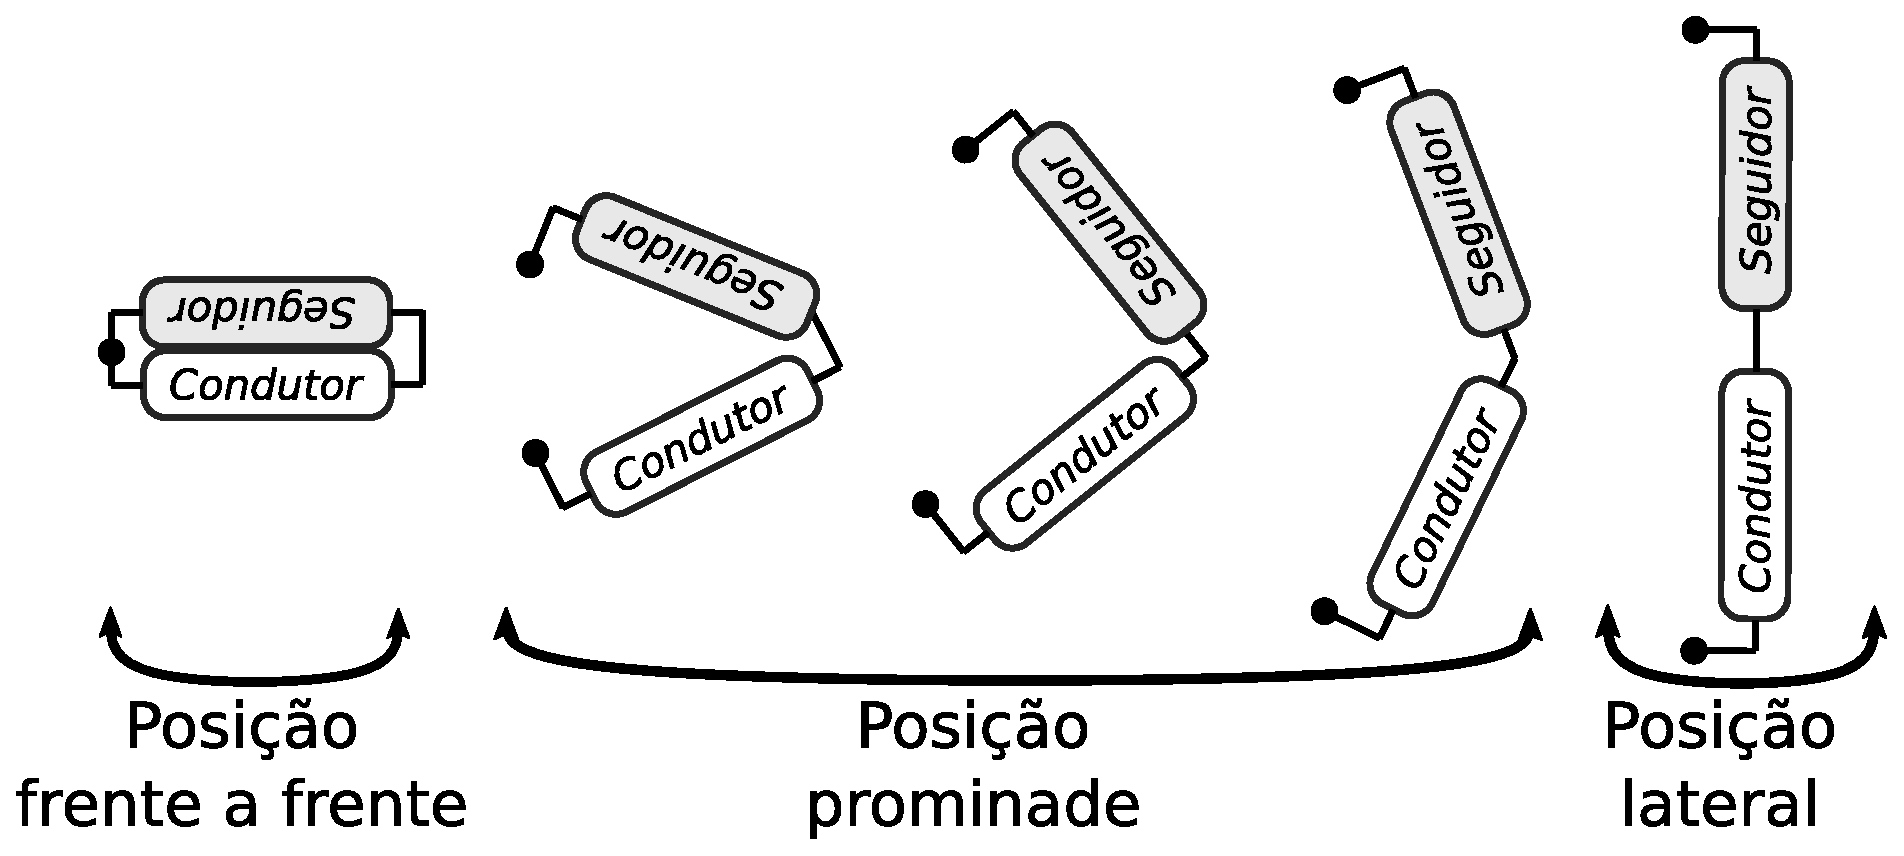
\includegraphics[width=0.8\textwidth]{chapters/cap-normas/desenhando.eps}
\caption{Transição do abraço na dança desde a posição fechada ate a lateral.}
\label{fig:desenhando}
\end{figure}

